%----------------------------------------------------------------------------------------
%	SLIDE 1.
%----------------------------------------------------------------------------------------
\begin{frame}
\frametitle{Overview}

\begin{block}{Types of limiting factors of rotation and radius}
	\begin{itemize}
		\item Limits for single stars (e.g. Kepler frequency, gravitational wave instabilities etc.)
		\item Absolute limits (e.g. General Relativity, Le Chateliér's principle, Causality etc.)
	\end{itemize}
\end{block}

\begin{columns}
\begin{column}{0.33\textwidth}
	\begin{figure}
		\centering
		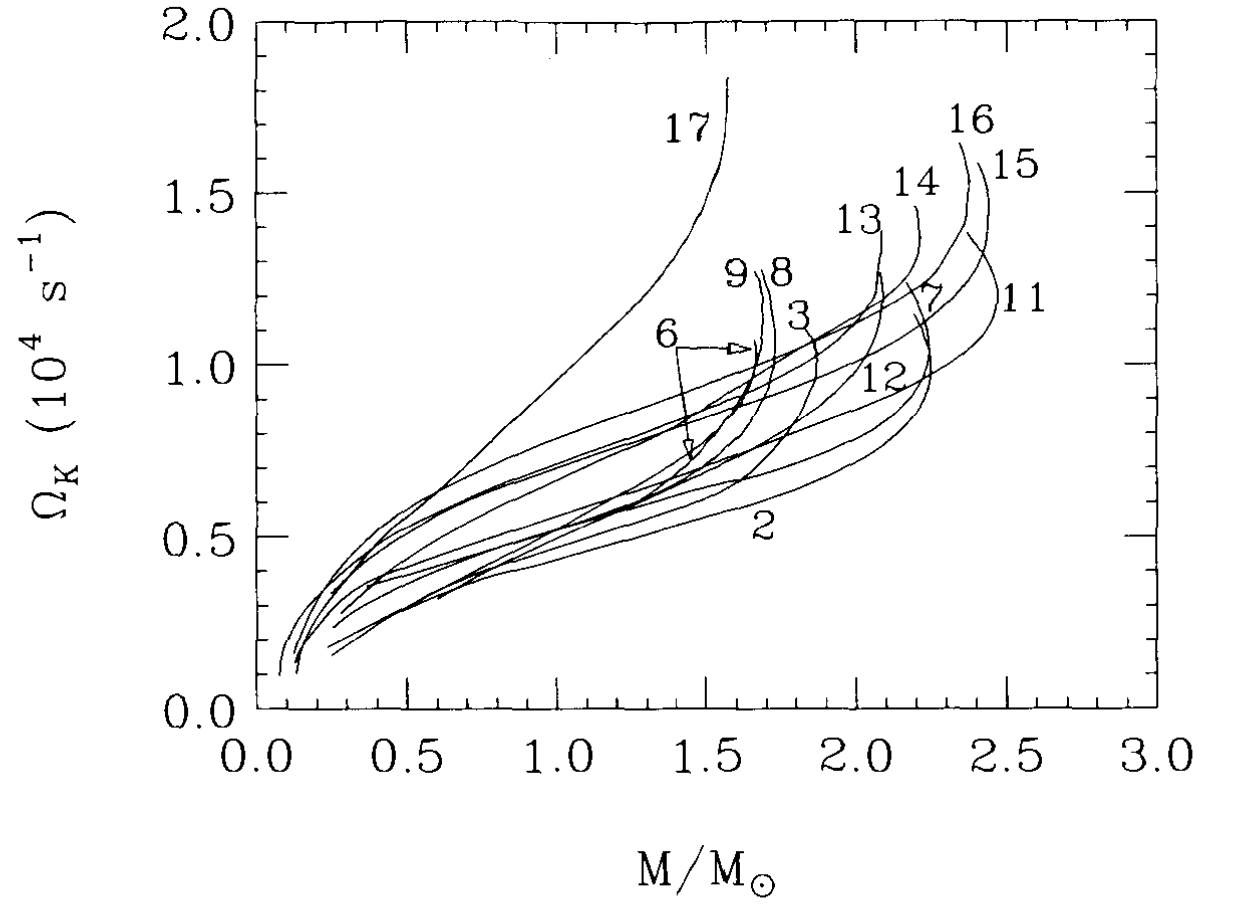
\includegraphics[width=0.9\linewidth]{./images/ns-mass-omega_k.png}
	\end{figure}
\end{column}
\begin{column}{0.33\textwidth}
	\begin{figure}
		\centering
		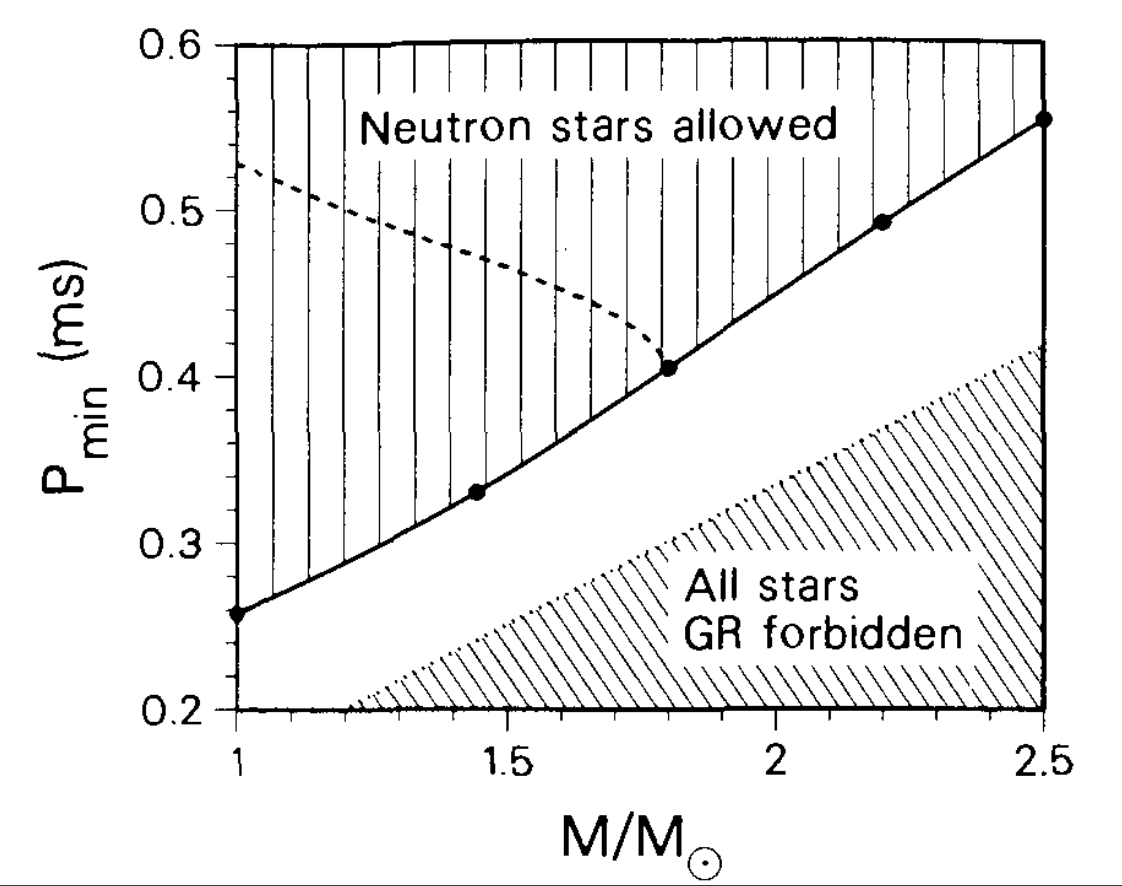
\includegraphics[width=0.9\linewidth]{./images/ns-mass-p_min.png}
	\end{figure}
\end{column}
\begin{column}{0.33\textwidth}
	\begin{figure}
		\centering
		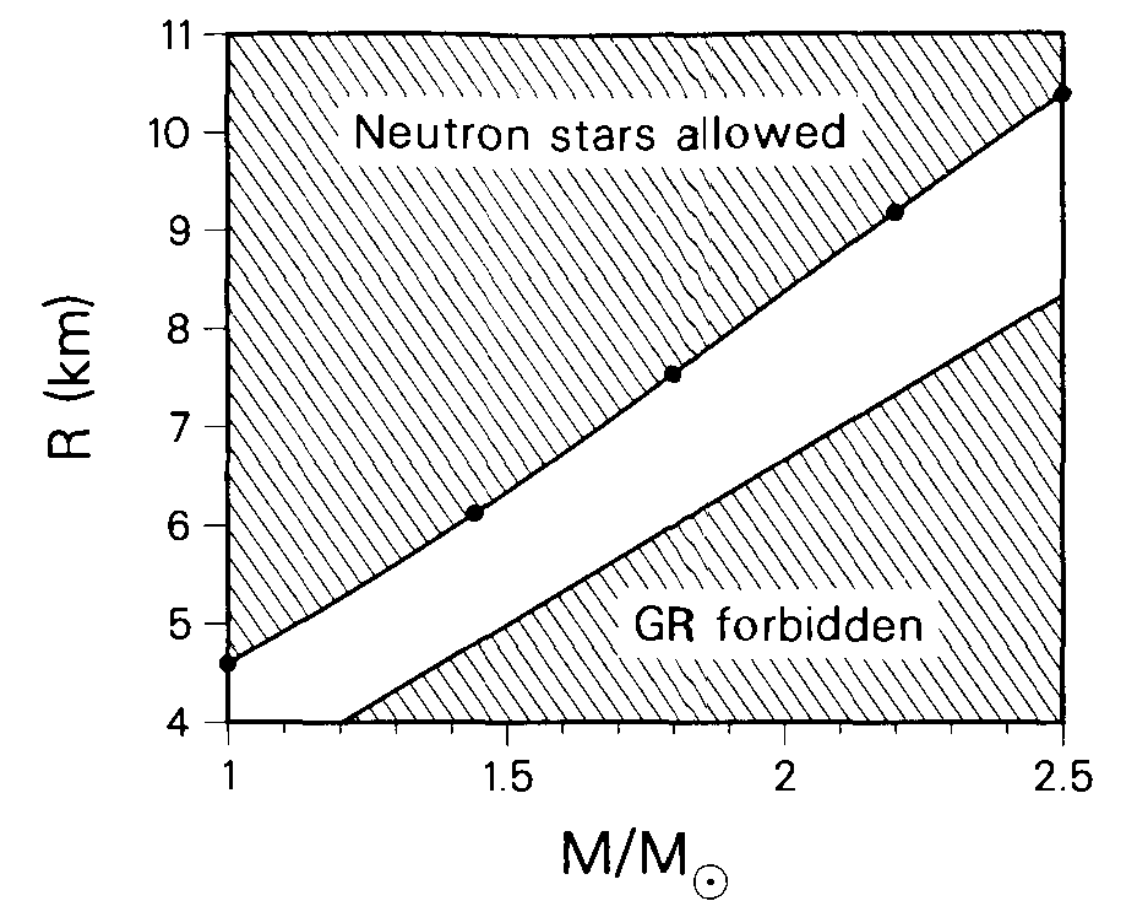
\includegraphics[width=0.9\linewidth]{./images/ns-mass-radius.png}
	\end{figure}
\end{column}
\end{columns}

\end{frame}